\chapter{Problem statement- State of the art} \label{ch:problem-statement}
\markboth{Problem statement- State of the art}{}

\paragraph{}
The key idea of this thesis is  an architecture that enables the implementation of economically attractive solutions that offer High-Availability to the IoT Edge Layer. It also proposes the most optimum way for critical infrastructure to be fault-tolerant, both in terms of services/functionality but also in terms of data quality (data integrity). However, preliminary discussions with experts of the domain (e.g. balena, EdgeX, blockchain domain)   led us to a more generic approach: That of resource sharing in a concept of share economy, in the domain of IoT Edge resources.

\section{The Sharing Economy}

Sharing Economy or “gig” economy is a relatively new term \cite{sharingeconomy},  popularised by famous companies like Airbnb or Uber. The idea is that services and goods can be distributed in a decentralized fashion, not by companies with employees but by private individuals who rent currently unused resources to other private individuals in a peer to peer fashion. In the above mentioned examples, individuals can rent their house (or part of it) when they don’t use it (Airbnb), or rent the “unused” seats of their cars, working, in essence, as taxi drivers whenever they choose to (e.g Uber, Lyft, etc.). Figure \ref{fig:sharing_economy} illustrates the concept of “Sharing Economy” for Airbnb which in essence provides access to Market to both parties of the value chain (Demand, Offer).

\begin{figure}[h]
    \centering
    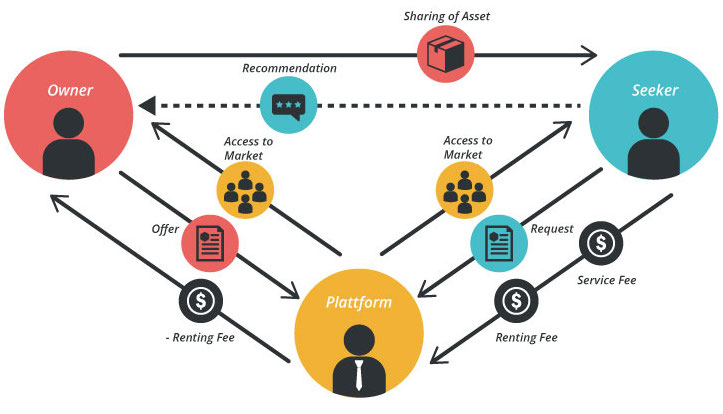
\includegraphics[width=0.9\textwidth]{images/sharingEconomy.jpg}
    \caption{The Sharing Economy Model;use-case of Airbnb\cite{airbnb}}
    \label{fig:sharing_economy}
\end{figure}

\section{Sharing Economy in the Internet of Things?}

We now attempt to apply the principles outlined in the above examples to the domain of IoT Edge resources.By tapping into that notion, IoT edge nodes could in fact share resources in order to provide services one to another, without necessarily belonging to the same stakeholder or even forming a federation. By incentivizing the IoT Edge Nodes to share resources, with a currency of sorts, we can foresee a \acrfull{m2m} marketplace, where IoT Edge Nodes will dynamically rent the resources that they need. In this scenario, an IoT Edge Node could provide Fault - Tolerance capabilities to nodes that are willing to pay for them. This could lead to a much more sustainable path of proliferating IoT Edge Computing , since it can considerably reduce the upkeep cost. There is no sense in owning Resources that you don’t use, only to anticipate a spike or an exception in the normal activity, but rather you can rent ad-hoc that extra computational power, if ever there is a need for it.

Indeed, the principle can be expanded with not only conventional computing resources, which we will define in Section \ref{st:edge-resources}  , but even with IoT specific “resources”. We argue that the handling of constrained devices (provision, management, data aggregation, semantic notation, metadata addition) can be viewed as a resource to be rented. Dynamic handover of Constrained Devices is an example of IoT specific “resources” that would provide value in a Fault-Tolerance scenario, as the Edge will not only need to take up any processing or decision making, but will also need to handle the data generators for a seamless transition from abnormal to normal operation. In essence, we envision 3rd party applications and/or services to run on the same physical Edge device. This physical Edge device will provide the needed resources to those applications so that they perform their tasks.

It is important here to underline that our solution is not about a multi-tenant platform, where different applications from different parties run on the same hardware. Each edge hardware is owned and operated by a distinct entity (an IoT platform provider for example), which is able to procure some resources to other parties so that they run a part (or even the entirety) of their application logic on the hardware. It is a dynamic relationship that can change rapidly due to the marketplace foundation and the open-ended offer and demand of resources (free market).

In other words, we believe that a platform for IoT Edge Computing as a service, is a much more interesting approach, while Fault - Tolerance is only a use case for it. It is interesting to note that there is not much bibliography concerning the high availability of edge computational resources by sharing them in a p2p economy, other than conventional methods such as backup systems. 

\section{MEC framework}

This idea has already been explored in the \acrfull{mec} framework\cite{7574435} which is believed to be critical for the introduction of 5G networks. Interestingly, while 4G is focused on delivering video content, 5G will focus on the growing M2M connections that is a direct result of the increase of IoT traffic and services\cite{cisco-visualise}. MEC offers cloud-computing capabilities in the RAN environment (Radio Access Network) while also offering an information technology service environment at the edge. They are characterized by very low latency, increased bandwidth and real-time access to radio networks. Moreover-and this is the part that is of interest to us- operators can open their RAN edge to authorized stakeholders so they can deploy their own applications and services toward their own subscribers (i.e private, enterprises and vertical solutions). MEC launched in 2014 by the European Telecommunications Standards Institute MEC Industry Specification Group (ISG) which by the time of writing has finished its work regarding the reference architecture for MEC.

\begin{figure}[ht]
    \centering
    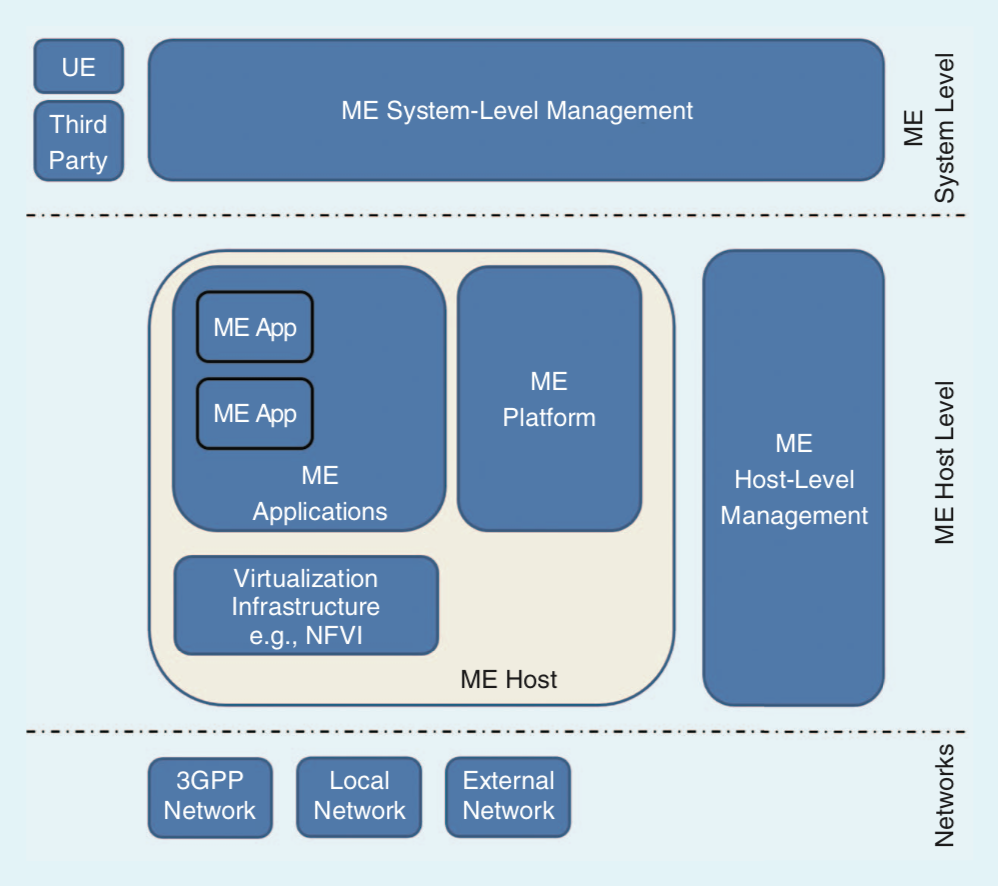
\includegraphics[width=0.9\textwidth]{images/mecarch.png}
    \caption{The High-Level Architecture of the MEC framework\cite{7574435}}
    \label{fig:mec}
\end{figure}

Figure \ref{fig:mec} illustrates the outline of the MEC reference architecture, where the top layer is the whole-system management layer that has an overall visibility of the system, while the bottom layer consists of the connectivity layer which includes all the possible connectivity protocols, from local area networks (LAN) to cellular internet. The layer in between, the host level features the ME platform and applications module, while also the virtualization environment on top of which the applications run. The ME platform is responsible for procuring to the ME applications, all the necessary resources and services they need, MEC can be seen as a cloud server running at the edge of a mobile network.

While MEC is extremely relevant to our solution and a cutting edge piece of standardized software, it diverges significantly from what we are proposing as it assumes trust between the MEC host and the MEC applications. Moreover, it is not designed for a dynamic supply and demand of Edge IoT Resources but rather for more longstanding federation agreements.  Finally, it is important to note that MEC was designed with telecommunications providers in mind, tailoring the architecture to their unique characteristics. Although more diverse deployments are discussed in MEC bibliography, it remains to see their actual effectiveness in regards to the private small-scale provider.

It is important to note that as the research continues on the solution, it is possible that the technology stack will swift to use MEC as the standardisation will improve the quality of the end result.


\section{Edge Resources} \label{st:edge-resources}

According to Mohammad Aazam et al.\cite{aazam2015dynamic} where they illustrate a dynamic resource provisioning mechanism for micro datacenters, computational resources are modeled by a set with the following elements \textit{R = [ CPU, storage, memory, bandwidth]}. In this research work, we will enrich the definition of Edge Resource with a superset of \textit{R}, \textit{R’ = [R, connectivity interface, uptime, battery power]}. This addition of two resources was necessary to model services that demand cyber physical I/O, as for example the handover of bluetooth sensors. The service-provider , apart from apparent CPU, memory \& storage resources, must also “spend” a bluetooth interface of the device. Depending on the use case, battery power or uptime could be an extremely valuable resource. In this context, uptime is defined as the total amount of time that the service will "run" (and which the service provider must ensure the \acrshort{qos}).

Note that the estimation, procurement , management and the monetary evaluation of resources is beyond the scope of this thesis. Nevertheless, the reader will find the above definition of an Edge Resource enlightening, as we dive into the architecture and implementation, in order to better grasp the positioning of our solution. 

Regarding resource management, there are works for efficient scheduling and adaptive offloading schemes that reduce complexity\cite{feng2017ave} with application to autonomous vehicles. Most researchers focus on the optimization of load distribution in a homogenous network of edge nodes that can work collaboratively and  can share the computational load. An example is Rogers Owen et al.\cite{rogers2012financial}, who present a methodology for resource allocation amongst Cloud computers (without resource prediction) while Deelman et al. present trade offs and performance metrics for various resource provisioning plans.  Zhen Xiao et al.\cite{xiao2012dynamic} present a resource allocation system that exploits virtualization technology in order to provision resources to services according to their needs, a vastly different model since it is apparent that it refers to the same physical Edge Node.

\section{ Fault-Tolerance/High-Availability}

High availability or Fault-Tolerance is a common cloud terminology and references to the ability of a system to continue it’s functionality in the case of a critical failure due to the replication of the services to multiple machines in distributed manner. While system redundancy has been partially solved by architectures such as the multi-region architecture, these solutions apply only to the cloud layer and usually the physical mainframes belong to the same stakeholder.

Our research has indicated that fault-tolerance at the edge layer is indeed a new concept, since the edge rarely performed any critical functionality, apart from aggregating sensor data and forwarding them to the cloud. A research study by D. LeClair et al. suggested that Edge Computing availability should surpass that of a data center(99.9\%) and should support at least five nines (99.999\%) availability\cite{ismail2015evaluation}.

Sudip Misra et al. propose an algorithm for fault-tolerance of IoT devices, regarding the routing of the IoT devices, using a Learning Automata as the core of the proposed algorithm \cite{misra2012adaptive}. Bukhary Ikhwan Ismail et al. propose a scheme utilizing the docker container technology as an Edge Computing (EC) platform, meeting a list of requirements that they defined as necessary: 1) deployment and termination; 2) resource \& service management; 3) fault tolerance and 4)caching \cite{ismail2015evaluation}.  The container technology  is in fact part of our solution as mentioned in Architecture Chapter \ref{ch:system-architecture}, but it’s only part of the solution, since the writers use docker swarm and a local docker image registry for each group of edge nodes. This creates multiple “single” points of failure, since a fail-over of the registry can result to the inability of the system to load new images. Details regarding the container technology and an in depth explanation will be given in Section \ref{st:containers}.

Such approaches are inherently different from our proposal since we will be targeting a broader spectrum of Edge devices, where trust between the actors (devices) is not a prerequisite. Our approach is closer to the architecture and principles of Helium \cite{helium}, a startup company which aims to create a decentralized network where nodes are compensated for providing Long Range Network Bandwidth to any sensor interested, as shown in Figure \ref{fig:helium}. The idea is to replicate the model of The Things Network\cite{ttn}, where people contribute their LoRa gateway to the network for anyone to use, but with the addition of an economic incentive to do so. Moreover, they use another communication protocol, called LongFi\cite{gemmell-2019}, a bi-directional data transfer system that is closely related to LoRa in terms of specifications (long range, low bandwidth). On top of it, the system is decentralized, meaning that the network is able to reach a consensus on who is actually providing wireless network coverage without depending on a centralized authority. Our work was greatly influenced by Helium, as network coverage could indeed be one of the resources that our architecture will be able to procure. An example, would be an Edge Device, that provides the activities of data aggregation and north-side forwarding, to any Constraint Device that is interested to pay for them (i.e as-a-service).

\begin{figure}[h]
    \centering
    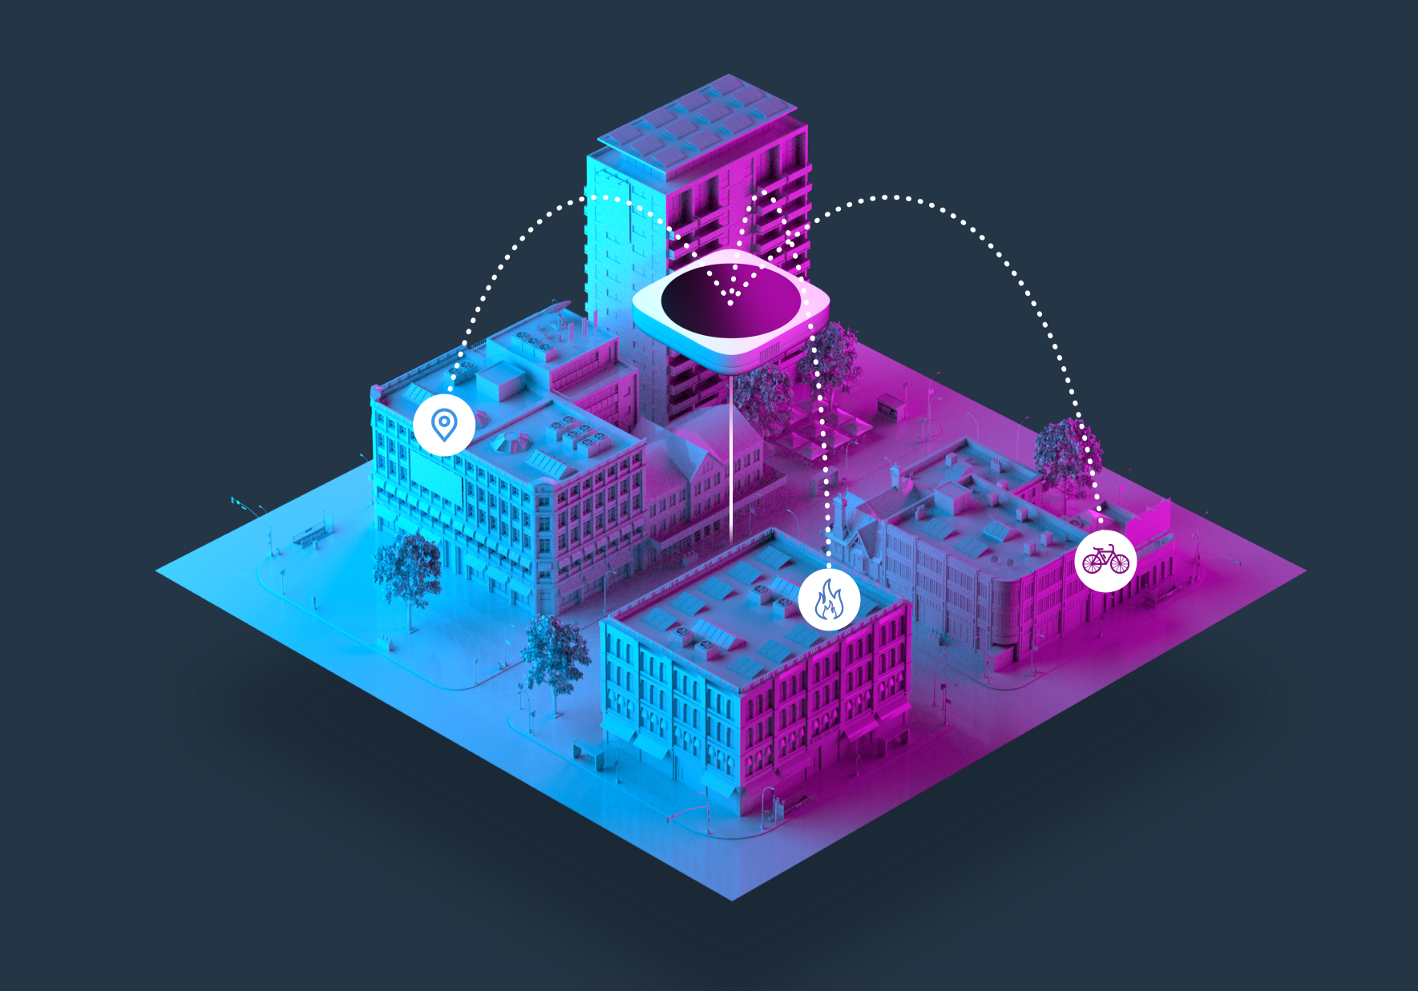
\includegraphics[width=0.9\textwidth]{images/helium.png}
    \caption{Illustration of a helium gateway providing coverage to IoT devices\cite{helium}}
    \label{fig:helium}
\end{figure}

\section{Storage Layer}

Another project that not only influenced the architecture and approach of our solution, but is also included as part of the proposed architecture, is Filecoin. Filecoin wants to turn the world’s unused storage into a decentralized algorithmic market, where anyone can offer his unused storage and be compensated for it, while clients can use the network to store their data. It is built on top of a very successful distributed file system called \acrfull{ipfs}, which is usually referred to as the decentralized HTTP. Although the project is still under heavy development, it is foreseen that the free-market economics of the project will render it a cheaper solution versus the already established storage solutions (such as Google Cloud, AWS, etc.). The Filecoin protocol will be described in depth in Section \ref{st:filecoin}. 


Decentralization offers the elimination of the single point of failure,  a point which is more interesting than it seems, even with the high-availability services that exist today. Recently, a user in twitter \cite{gigazine} mentioned that because of an AWS datacenter power failure (which was coupled with a failure of the on-site backup power generators), the entire datastore of his companies data was erased. Even though the data was restored, because of the timely backup routine, in different scenarios where the data influx is much greater (such as a typical IoT scenario), this power failure could create a hole in the historical data of the platform. Finally, an interesting argument for decentralization is that censorship is impossible to be conducted in a decentralized ecosystem. We must remember that although the Cloud providers have a strong incentive to act in a faithfuly, they are in fact in control of the data we store, a point which depending on the application vertical can have more or less importance, especially in privacy sensitive scenarios (e.g healthcare technology).

Taking into account our need for a storage network, as a means to reduce storage costs, and decentralization there are a couple of projects that we could potentially use, namely: 1)StorJ\cite{storj}, 2)Sia\cite{sia} and 3)Filecoin\cite{filecoinlabs}. We outline some of their attributes and we conclude on why Filecoin was chosen.

\begin{enumerate}
    \item \textbf{Sia:}
    
Sia is an early project that started back in 2013 at HackMIT and officially launched in 2015. It aims to leverage underutilized hard drive capacity around the world to create a data storage marketplace which is more efficient and cheaper to current solutions. They have a working product and have interesting design features. They have preference for the Proof-of-Work(PoW), have their own ASIC chips for Siacoin mining and utilise file contracts to set rules and requirements for storage (similar to a smart contract). Their Proof of Storage algorithm is utilised to further protect and validate proofs and file contracts on the network.

\item \textbf{StorJ:}

Another decentralised storage project, built on the Ethereum network that has quite a lot of community users and is dedicated to the open-source ethos. Storj is a platform, cryptocurrency, and suite of decentralized applications that allows you to store data in a secure and decentralized manner.

Their technology revolves around file sharing, similarly to how torrents work and separates parts of the files to users in the network. When a user wants the file, he requests it and Storj uses a distributed hash table to locate all the shards and piece them together. These files are also encrypted before sharing and the person uploading it has their own private key to validate ownership. The other entity of the company Storj Labs is the for-profit side that rents out it’s network to thousands of users and charges for the network usage. This is a slightly more centralised model and competes with the likes of Dropbox and Google Drive. They also have partnerships with Microsoft Azure and Heroku to deploy some of their development tools which is a great initiative for the open source developer ecosystem.

\item \textbf{Filecoin + IPFS:}

The InterPlanetary File System (IPFS)\cite{ipfslabs} is a protocol started by Protocol Labs to create a new way to server information on the web. Currently the Internet works off a location based addressing where you go to a URL like medium.com which has an IP of X.X.X.X and then you get served your articles. These URL’s are pointed to certain servers around the world. Instead, what IPFS does is serving information based on what it is as opposed to where it is (location). With their routing algorithms, a user can choose where he gets the content from and he can set his privacy on what peers/nodes he trusts to receive the files from. A high level overview of the protocol is shown in Figure \ref{fig:ipfs} \cite{ipfslabs}.

\begin{itemize}
    \item  Hash addressing makes the content immutable. It does not disappear like current HTTP protocol.
    \item Saves bandwidth by collecting content from multiple nodes and pieces instead of from one server.
    \item Access to content “offline” or in low connectivity 3rd world or rural areas, in the same sense that git works offline.
    \item Censorship resistant.
    \item It is built around the decentralisation ethos.

\end{itemize}

To further utilise this technology, Filecoin was proposed as a way of creating a decentralised storage network by using the unused storage lying around and incentivize users to be part of the sharing economy through Filecoins (FIL) by using the IPFS protocol. The project is still under heavy development, so it will be interesting to see how they build with their proposed Proof of Space and Proof of Replication consensus algorithms, which will be discussed further in the Architecture Chapter \ref{ch:system-architecture}. 
\end{enumerate}

\begin{figure}[h]
    \centering
    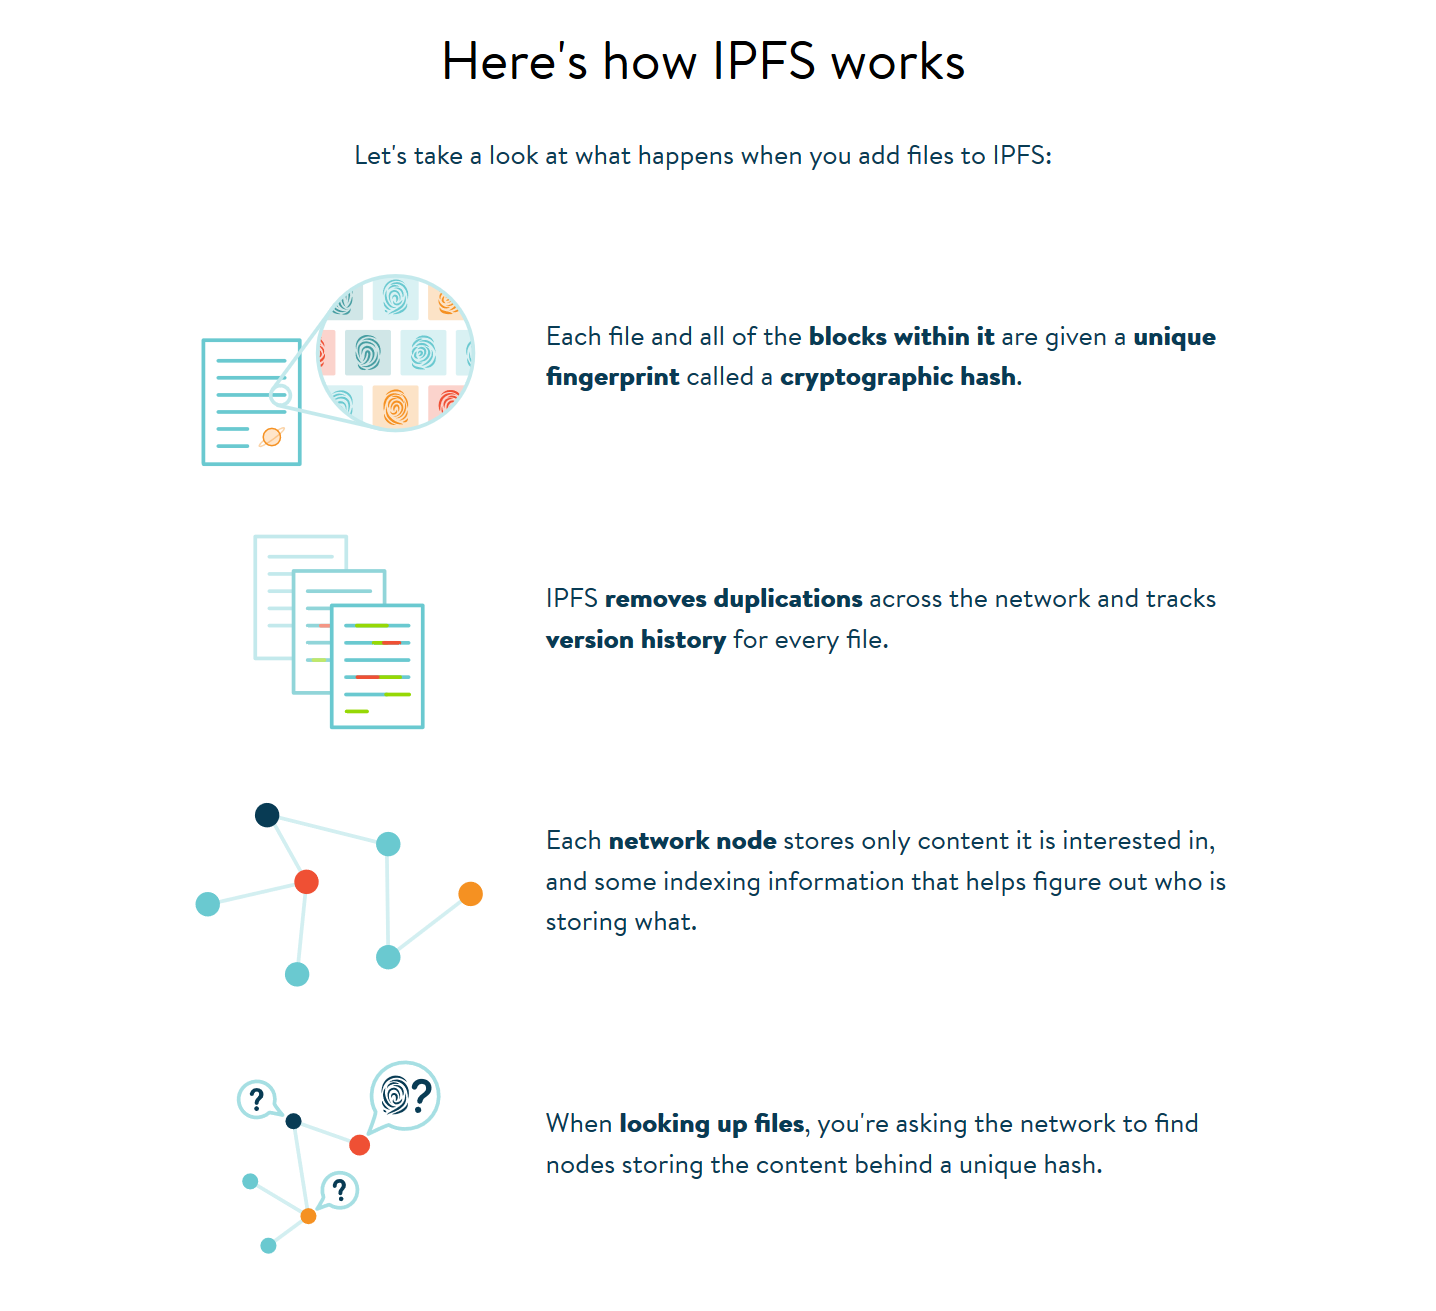
\includegraphics[width=0.9\textwidth]{images/ipfs.png}
    \caption{High-Level overview of the IPFS protocol \cite{ipfslabs}}
    \label{fig:ipfs}
\end{figure}

\subsection{Why Filecoin was chosen}

Filecoin was chosen because it already utilizes a protocol that has been used for several years, establishing itself as the standard for the distributed storage of files in the blockchain community. Moreover, Protocol Labs is a proven development team, having already developed IPFS itself, illustrating serious technical capabilities as also a thorough technical approach. Finally, the development of Filecoin is considerably slower than the other projects, as the team establishes the basic research on top of which the technology will be built. The research based orientation and the technical aspects of the Filecoin whitepaper\cite{filecoin-whitepaper} show great promise and care for the engineering quality of the product, aspects that are highly valued in a domain as pioneering as blockchain. We wanted to integrate in our architecture, a solution that can be viewed for the long-term, supporting in the meantime its development by being early adopters and contributors.

\subsection{Data Integrity}

Data integrity is the overall completeness, accuracy and consistency of data, which means that the data must be collected and stored in an tamper-proof and undeletable fashion. This is extremely important for certain problem domains, such as critical infrastructure. Data Integrity can be achieved by enforcing the Edge systems to digitally sign the sensor data while maintaining an end-to-end cryptography between the sensor and the Edge. Moreover, data integrity dictates that data storage is inherently high-available, meaning that the data storage is equally important as the data collection.

The problem of data integrity has been extensively studied in all traditional computing and communication systems and some preliminary results exist for sensor networks\cite{acharya2008data}. Data integrity became extremely relevant after the trend of storing data on the cloud. While it is easy to check data integrity after completely downloading the data to be checked, downloading large amounts of data just for checking data integrity is a considerable waste of bandwidth. Moreover, remote data integrity validation was firstly introduced using the RSA (Rivest–Shamir–Adleman) based methods and afterwards using a challenge-response model, by Shah et al\cite{shah2007auditing}. In the second model, the user challenges the data storage computer system to respond with a succinct proof which will show that indeed he is storing the data. The simplest of such methods is the division of the data into blocks and the hashing them, but there are other methods with increased efficiency\cite{kumar2011data}.

Blockchain technology is a recent candidate for this issue, as it combines the characteristics of an immutable record with a distributed database. There are currently two mains usages of blockchain to enforce data integrity on the data pipeline. 

\begin{enumerate}
    \item Store data directly on the blockchain, extremely secure but raises a lot of issues regarding scalability and performance. Infeasible for large streams of data.
    \item Package data and store a hash on the blockchain. Thus an immutable succinct record of that data is created. A user needs both the data and the hash to verify the correctness of the data.
\end{enumerate}

\section{Use Cases}

As the thesis attempts to introduce an innovative concept in a new domain, it is pertinent to introduce two (2) use cases that will help the reader to understand the usability of the proposed architecture. The first use-case is the one that was chosen to be the objective of the proof of concept implementation, the fault-tolerance scenario. The second is more generic, illustrating the ad-hoc provision of services.

\subsection{Use Case 1: Fault-Tolerance}

The fault tolerance use case was inspired by a scenario, local to the university of Patras. Near the university, there is a bridge called “Rio-Antirio bridge” or as officially named “Charilaos Trikoupis Bridge”. It is one of the world's longest multi-span cable-stayed bridges and the longest of the fully suspended type, as shown in Figure \ref{fig:riobridge}. A true marvel of engineering, it has 4  pillars over an exceptionally difficult area with numerous challenges, namely the frequent earthquakes, the weak ground and the depth of the gulf. A bridge of this magnitude, houses numerous sensors which aid the bridge operators into verifying the integrity and safety of the bridge, while also acting proactively to any challenge that may rise \cite{rion-antirion-bridge}. It is safe to presume that there is an Edge system that aggregates this data, maybe performs some processing and analytics and then feeds the cloud system that offers the rest of the services to the operators.

\begin{figure}[h]
    \centering
    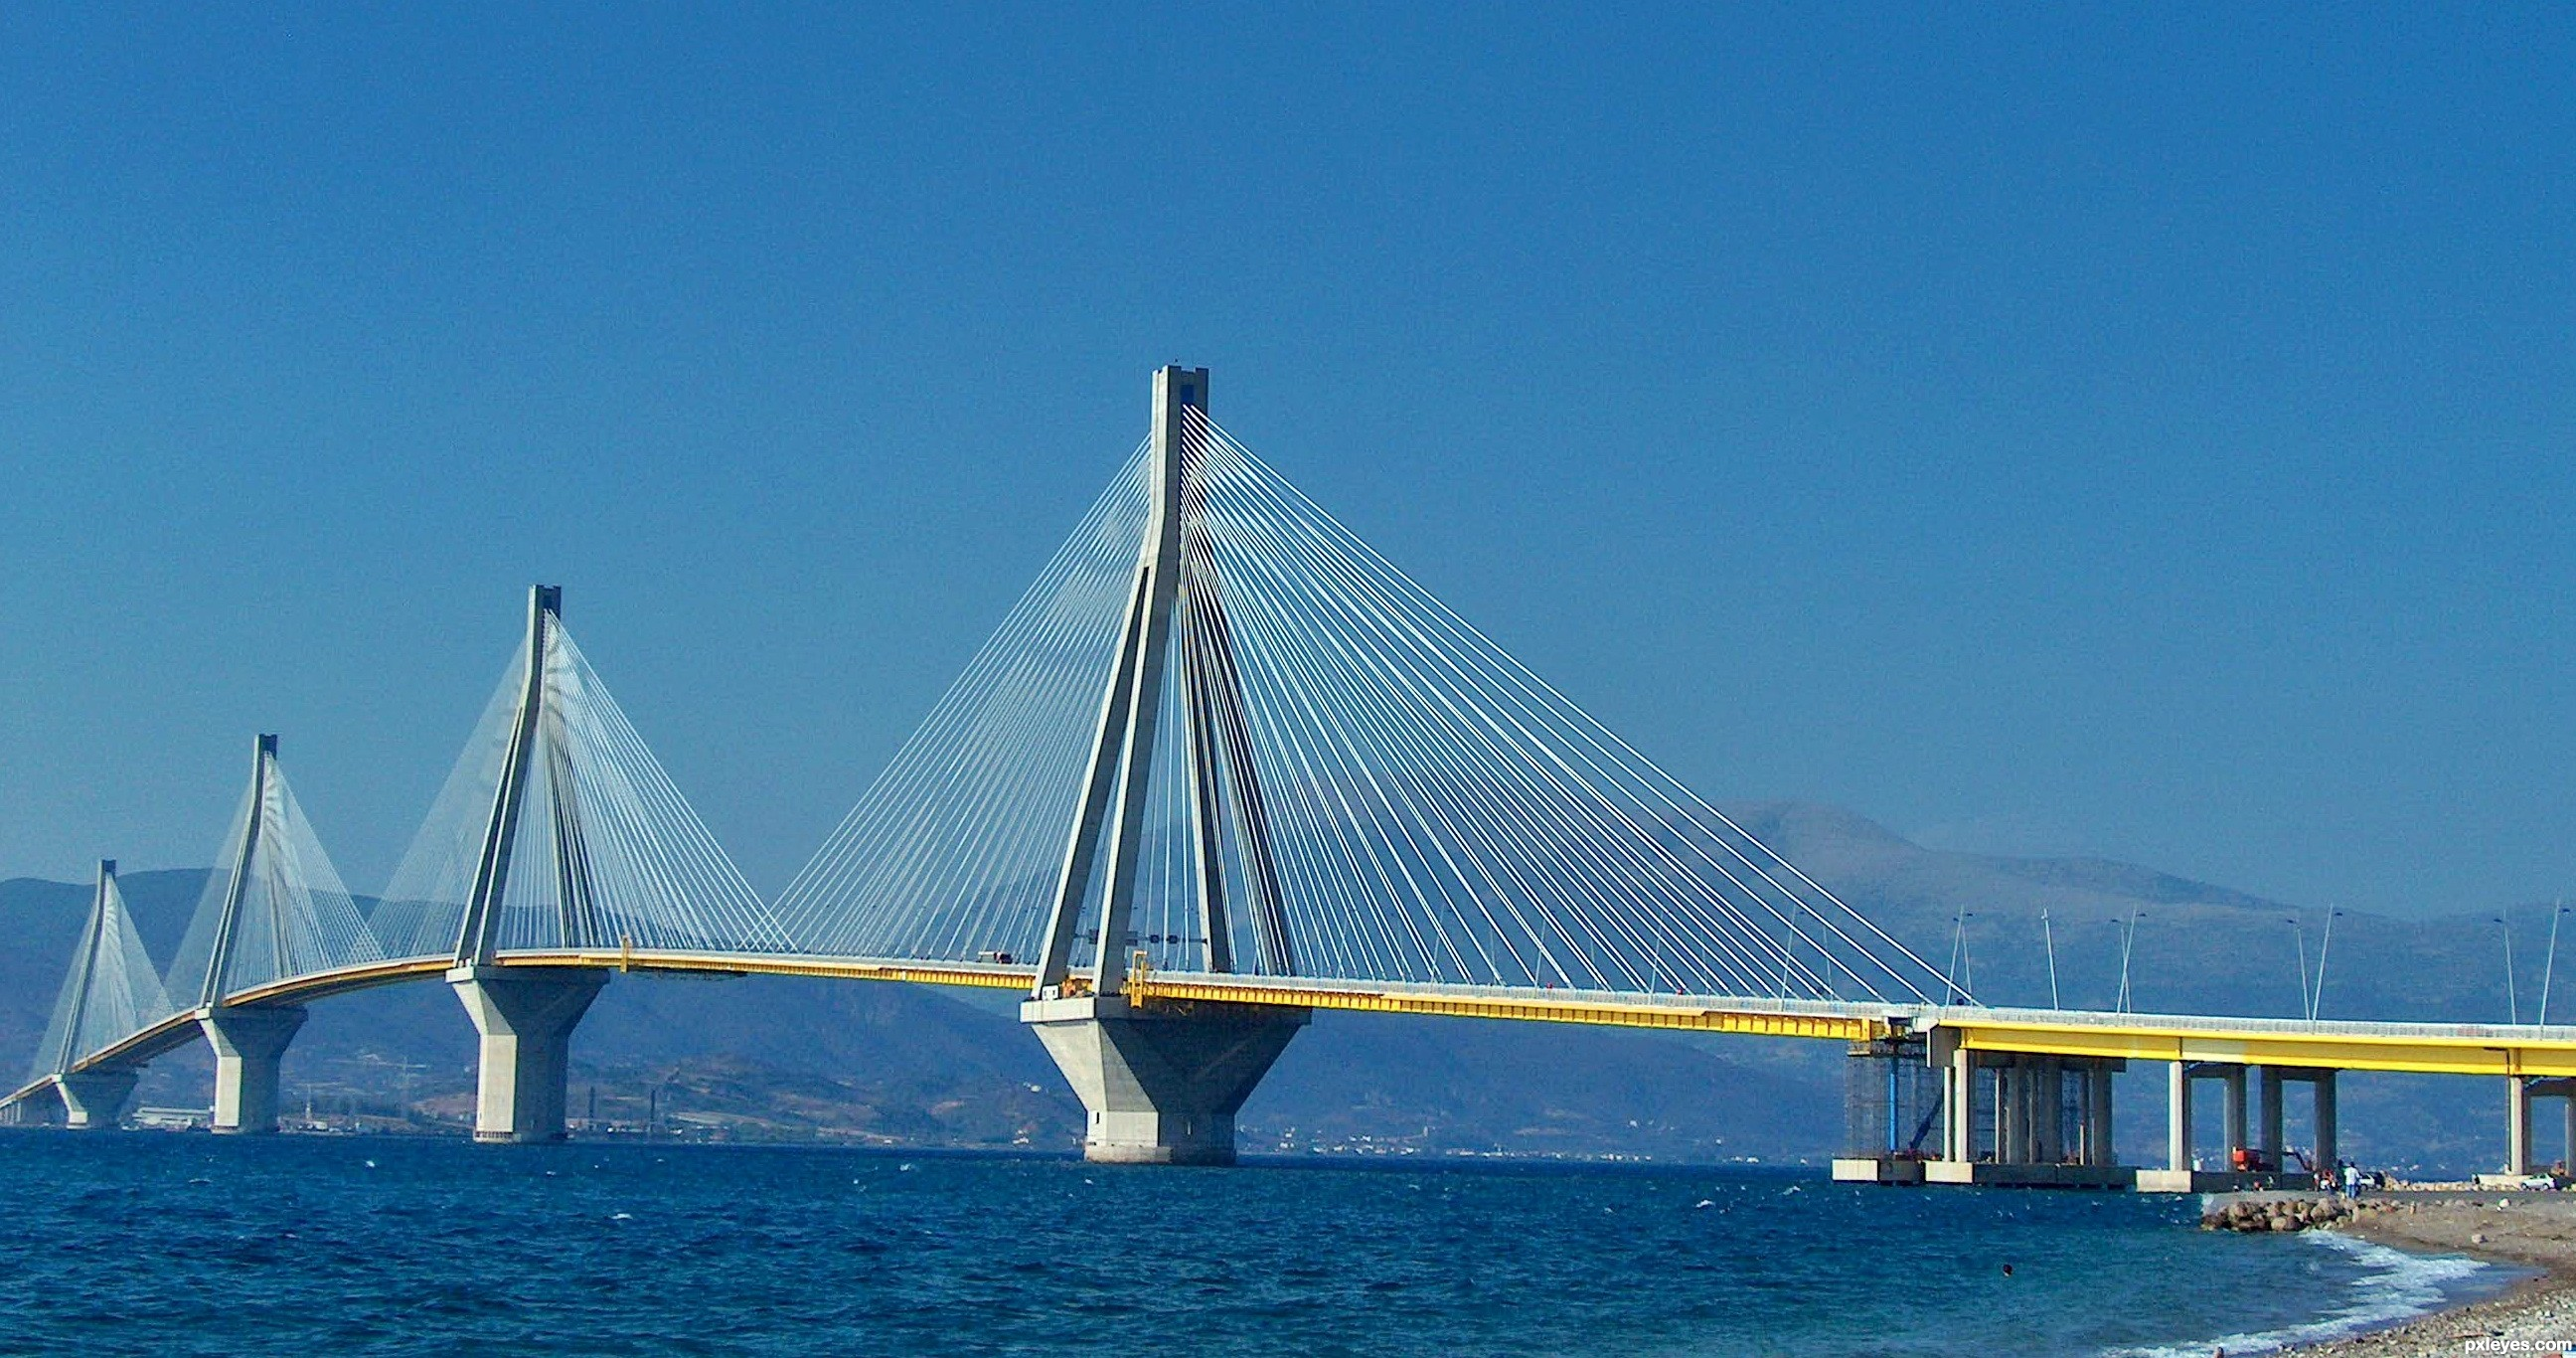
\includegraphics[width=0.6\textwidth]{images/rio-bridge.jpg}
    \caption{The Rio-Antirio Bridge in Western Greece \cite{riowiki}}
    \label{fig:riobridge}
\end{figure}

It is also safe to presume that there are protocols in place for the case that the computer system (“Edge”) fails and the operators are left effectively blind. What would happen if the University of Patras, which is nearby, could in fact jump in with and offer a micro-datacenter, in order to take over the bridge management until the issue is fixed? Due to the extreme locality of the two computer systems, University of Patras can still be considered as “edge” for the Rio-Antirio bridge IoT system. In Figure \ref{fig:rio-map} we see a map overview of the scenario, where the university is clearly indicated by the blue market at the bottom, while the Rio bridge side at the top. The black line that connects the two landmarks is approximately 2.3km, illustrating the extreme locality of the two Edge computers.

\begin{figure}[ht]
    \centering
    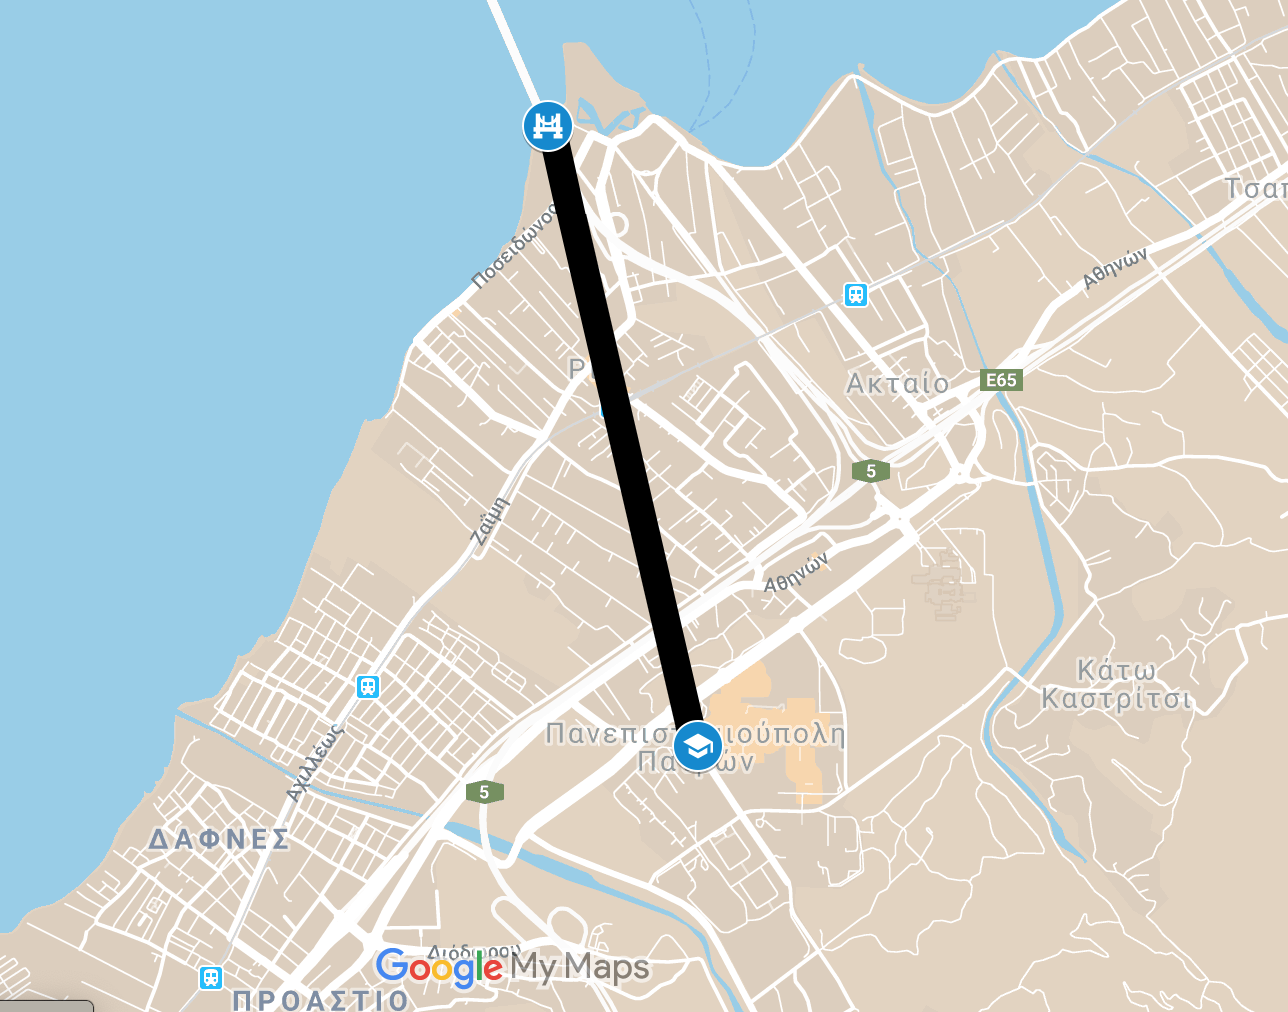
\includegraphics[width=0.6\textwidth]{images/usecase1map.png}
    \caption{A map illustrating the close proximity of the Bridge and the University}
    \label{fig:rio-map}
\end{figure}

The handover of the sensors and all relevant functionality would happen automatically, as soon as a failure was detected by the platform at the University of Patras. The two edge systems would have a priori signed a digital contract, containing all the necessary information, such as needed resources, services, protocols, contract activation conditions and of course payment. The goal is for this dynamic federation to happen in an automated fashion, on a platform that will guarantee the Quality of Service needed for such an important critical infrastructure.

\subsection{Use case 2: Drone passage over IoT Edge Nodes}

The second use-case is more generic in order to showcase the robustness of the architecture over a broad spectrum of issues. In this use-case, we envision a drone that flies over a predetermined route in order to perform some specialized functionality. This drone activity is characterized by three important aspects: 

\begin{enumerate}
    \item  It generates a large number of raw data (such as video feed).
    \item It needs to perform pre-processing before sending it to the cloud due to bandwidth limitations.
    \item Limited battery capacity.
\end{enumerate}

It is apparent that the processing of the data can not be done on the drone itself as the battery would be impossible to realistically handle the consumption demands of the CPU, coupled with the inherent power consumption hungry nature of a drone (i.e the motors). For this reason, the drone knowing the route beforehand, has reached an agreement with a number of edges that are geographically near the route in order to offload the pre-processing and cloud forwarding to them. The drone would then simply fly and stream the data to them, while the IoT Edges will know exactly what to do and what specifications their services need to meet. The streaming could use a low-range protocol such as WiFi or Bluetooth. Figure \ref{fig:drone_map} illustrates an autopilot program for drones \cite{ardupilot}, which enables drone to fly over a predetermined route.

\begin{figure}[h]
    \centering
    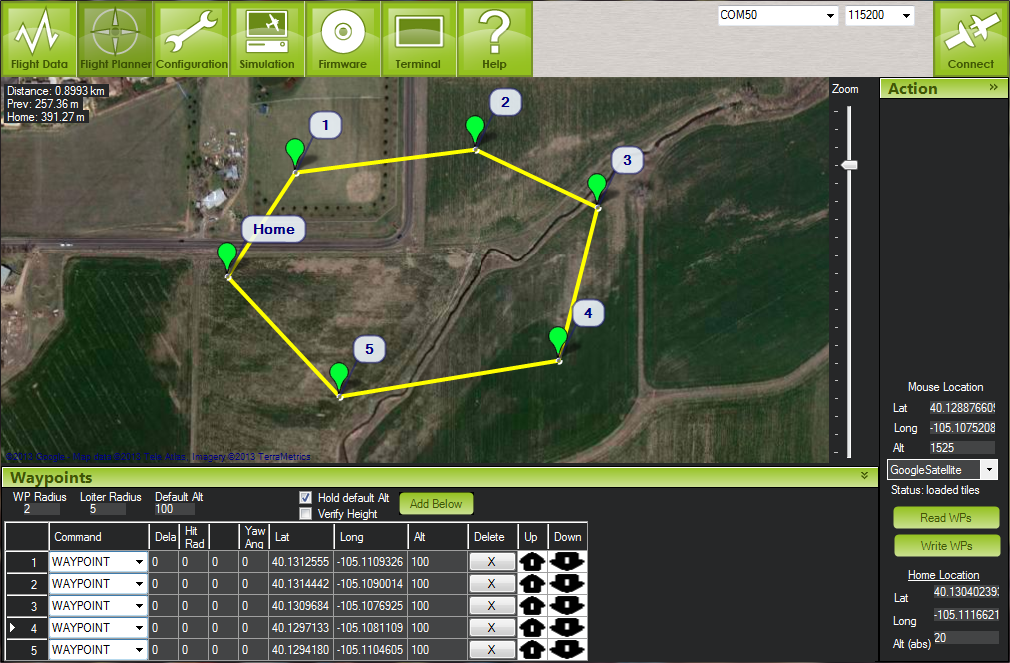
\includegraphics[width=0.7\textwidth]{images/droneroute.png}
    \caption{The GUI of a Drone route mapping software\cite{ardupilot}}
    \label{fig:drone_map}
\end{figure}